\documentclass[11pt,a4paper]{article}

% -----------------------------------------------------------------------
% Packages
% -----------------------------------------------------------------------
\usepackage[margin=2.5cm]{geometry}
\usepackage{hyperref}
\usepackage{booktabs}
\usepackage{graphicx}
\usepackage{amsmath}
\usepackage{amssymb}
\usepackage{array}
\usepackage{xcolor}
\usepackage{colortbl}
\usepackage{multirow}
\usepackage{microtype}
\usepackage{natbib}
\usepackage{caption}
\usepackage{subcaption}
\usepackage{float}
\usepackage{enumitem}
\usepackage{url}
\usepackage{parskip}

\hypersetup{
  colorlinks=true,
  linkcolor=blue!60!black,
  citecolor=blue!60!black,
  urlcolor=blue!60!black,
}

% Colour palette for heatmap cells (defined here for use in tables)
\definecolor{heatH}{rgb}{0.18,0.55,0.34}   % dark green: 1.0
\definecolor{heatM}{rgb}{0.60,0.80,0.48}   % light green: 0.875–0.944
\definecolor{heatL}{rgb}{0.98,0.82,0.38}   % amber: 0.714–0.857
\definecolor{heatR}{rgb}{0.90,0.35,0.24}   % red: <0.714
\definecolor{deductH}{rgb}{0.90,0.35,0.24} % deduction red

% -----------------------------------------------------------------------
% Title block
% -----------------------------------------------------------------------
\title{\textbf{Text2WetLab: Benchmarking Large Language Model Agents\\
on Opentrons OT-2 Protocol Generation}}

\author{
  Niall O'Leary$^{1}$ \quad
  Evan O'Leary$^{1}$ \quad
  Mohammed Alshehri$^{1}$ \quad
  Laurence Sturdy$^{1}$
  \\[6pt]
  \small $^{1}$Independent
  \\[4pt]
  \small \texttt{text2wetlab@proton.me}
}

\date{October 2026}

% -----------------------------------------------------------------------
\begin{document}
\maketitle
\thispagestyle{empty}

% -----------------------------------------------------------------------
\begin{abstract}
We introduce \textbf{Text2WetLab}, a benchmark for evaluating large language
model (LLM) agents on the task of generating executable Opentrons OT-2
liquid-handling protocols from plain-English instructions.
The benchmark comprises seven tasks ranging from a trivial two-well
transfer to a 48-sample magnetic-bead RNA extraction derived from a
published COVID-19 diagnostic paper.
Each submission is graded by a \emph{dual-layer} pipeline: a deterministic
layer (Opentrons simulator plus state-trace checks) and a rubric-based LLM
judge that scores tacit wet-lab knowledge.
We evaluate three frontier models---Anthropic Opus~5.5, Sonnet~5.5, and
Fable~5.1---using pass@1 across 21 trials executed in Modal cloud sandboxes.
All 21 submissions passed the deterministic layer (sim\_pass\,=\,1.0),
confirming that syntactic and structural correctness is largely a solved
problem.
Score variation arose entirely from the LLM judge.
Opus~5.5 achieved the highest mean reward (0.935), Sonnet~5.5 was the most
cost-efficient (0.910 mean at 33\,\% of Opus cost), and Fable~5.1 scored
0.882.
Cross-cutting failure modes include: a \emph{phantom mix} hallucination in
which two models added an unrequested \texttt{mix\_after} step to competent
\emph{E.~coli} cells, a \emph{cross-contamination} tip-reuse error in
colony PCR invisible to the deterministic grader, and a \emph{universal
elution-volume error} in RNA extraction (100\,\textmu L aspirated instead of
80\,\textmu L, risking pellet carry-over in a clinical-extraction protocol).
These results demonstrate that LLM agents can reliably produce runnable
OT-2 code but still fail on tacit wet-lab safety knowledge that only the
rubric layer can detect.
\end{abstract}

\tableofcontents
\newpage

% -----------------------------------------------------------------------
\section{Introduction}
\label{sec:intro}
% -----------------------------------------------------------------------

Laboratory automation is increasingly within reach of biologists who do not
have a programming background.
Platforms such as the Opentrons OT-2~\citep{opentrons2019ot2} provide
open-source liquid-handling robots that accept Python scripts using a
structured API, offering a concrete, machine-verifiable output format for
an NL-to-code generation task.
At the same time, recent frontier LLMs have demonstrated strong code
generation and instruction-following capabilities, raising the question of
whether a plain-English description of a laboratory procedure is sufficient
to generate a safe, runnable protocol without manual programming.

The gap between ``runs without error'' and ``is safe to execute'' is the
central motivation for this work.
A protocol that passes the simulator can still:
(i)~reuse a tip across biologically distinct samples, causing
cross-contamination;
(ii)~mix competent cells at a step where the protocol explicitly says not
to; or
(iii)~aspirate from the wrong depth, risking pellet carry-over in a
magnetic-bead purification.
None of these faults is visible to a compiler or a syntax checker.
They require domain knowledge about wet-lab practice.

We make the following contributions.

\begin{enumerate}[leftmargin=*]
  \item A \textbf{seven-task benchmark suite} (Text2WetLab) spanning four
    orders of biological complexity, from a two-well pipetting exercise to
    a 48-sample viral RNA extraction, with reproducible task definitions
    grounded in published experimental protocols.

  \item A \textbf{dual-layer grading pipeline} combining a deterministic
    Opentrons-simulator layer with a structured LLM-judge layer, and an
    empirical demonstration that the LLM layer is necessary: the 11 rubric
    deductions in our results would all have been invisible to deterministic
    grading alone.

  \item \textbf{Per-task, per-rubric failure attribution} for three frontier
    models across 21 trials, characterising four distinct failure modes.

  \item A \textbf{cost-efficiency analysis} showing that Sonnet~5.5 achieves
    97.3\,\% of Opus~5.5's performance at 33\,\% of the cost.
\end{enumerate}

Anthropic's Model Hardware Standard (MHS)~\citep{anthropic2026mhs}
provides a useful framing: safe AI deployment in physical environments
requires that models understand not just the formal specification of a task
but also the implicit safety invariants of the domain.
Text2WetLab operationalises this requirement in the specific context of
laboratory robotics.

% -----------------------------------------------------------------------
\section{Related Work}
\label{sec:related}
% -----------------------------------------------------------------------

\paragraph{Agent benchmarks for science and robotics.}
AGEIS~\citep{ageis2025} benchmarks LLM agents on laboratory AI tasks
including instrument control and experimental design, providing a broader
multi-domain view; Text2WetLab complements it with a fine-grained focus on
a single instrument class and on tacit wet-lab safety.
Libero~\citep{liu2023libero} benchmarks robot learning on a suite of
manipulation tasks; our work shares its emphasis on task diversity and
quantitative per-task attribution, but targets code generation rather than
imitation learning.
PyLabRobot~\citep{wierenga2023pylabrobot} provides an open-source Python
interface to multiple liquid-handling platforms and demonstrates the demand
for programmatic control of lab robotics.

\paragraph{Evaluation frameworks.}
Harbor~\citep{harbor2026} is an open-source framework for running LLM
agent benchmarks in reproducible sandboxed environments using Modal, Daytona,
and other cloud back-ends.
Text2WetLab tasks are structured as Harbor tasks, making them directly
runnable by any team with access to an Anthropic API key.
Claude Code~\citep{anthropic2026claudecode} is the agent used to drive
protocol generation in all our trials.

\paragraph{NL-to-code benchmarks.}
Text2SQL~\citep{yu2018spider} established the paradigm of evaluating NL-to-
structured-code translation with execution-based grading.
Text2WetLab extends this paradigm to a physical-world domain where
correctness depends not only on whether the code runs but on whether the
resulting physical actions are safe and scientifically valid.

\paragraph{Protein and biological benchmarks.}
ProteinGym~\citep{notin2023proteingym} benchmarks models on protein fitness
prediction using high-throughput experimental data.
It informs our design in its emphasis on grounding evaluation in real
experimental outcomes rather than proxy metrics.

% -----------------------------------------------------------------------
\section{Benchmark Design}
\label{sec:design}
% -----------------------------------------------------------------------

\subsection{Task Suite}
\label{sec:tasks}

Table~\ref{tab:tasks} describes the seven tasks.
They were selected to span a range of biological procedure types, pipeline
complexity (number of steps, labware count, and required domain knowledge),
and grading strategy.
Two tasks (\texttt{a1-a12-100ul}, \texttt{split-200ul-two-wells}) were
hand-written as controlled baselines.
Five tasks are grounded in published experimental papers, with the
RNA-extraction task using the exact instrument script published by the
Amsterdam UMC Leiden clinical laboratory as the oracle~\citep{steur2021hulp}.

\begin{table}[H]
\centering
\caption{Text2WetLab task suite. Complexity is rated Low/Medium/High/Expert.
``Grader'' indicates which layer(s) judge the task beyond the simulator gate.
``Source'' is the origin of the task specification.}
\label{tab:tasks}
\footnotesize
\begin{tabular}{lllp{5.2cm}l}
\toprule
\textbf{Task} & \textbf{Complexity} & \textbf{Grader} & \textbf{Instruction (NL)} & \textbf{Source} \\
\midrule
\texttt{split-200ul-two-wells}        & Low    & Det.\ + Judge & Move 200\,\textmu L from reservoir into two wells.
                                                                & Handwritten \\
\texttt{a1-a12-100ul}                 & Low    & Det.\ + Judge & Add 100\,\textmu L from a 1-well reservoir to wells A1$\to$A12.
                                                                & Handwritten \\
\texttt{ampure-bead-cleanup}          & Medium & Det.\ + Judge & 0.8$\times$ AMPure XP cleanup of 50\,\textmu L PCR products
                                                                  (bead incubation, 2 EtOH washes, 5\,min dry, 50\,\textmu L elution).
                                                                & Pioneer NGS \\
\texttt{colony-pcr-screening}         & Medium & Det.\ + Judge & Add 18\,\textmu L master mix, then 1\,\textmu L colony DNA and
                                                                  1\,\textmu L primers per well.
                                                                & Slowpoke~\citep{slowpoke2025}, APEX~\citep{apex2024} \\
\texttt{ecoli-heat-shock-transformation} & Medium & Det.\ + Judge & Transform competent \textit{E.~coli} with 2\,\textmu L plasmid per tube,
                                                                      heat-shock 42\,\textdegree C/45\,s, add 250\,\textmu L SOC.
                                                                & APEX~\citep{apex2024} \\
\texttt{golden-gate-assembly}         & High   & Det.\ + Judge & Full Golden Gate assembly: PCR, DpnI digest, cleanup, reaction setup,
                                                                  thermocycler, transformation.
                                                                & AssemblyTron~\citep{assemblytron2023} \\
\texttt{opentrons-rna-extraction}     & Expert & Det.\ + Judge & 48-sample magnetic-bead viral RNA extraction from PLOS ONE 2021 paper.
                                                                & HULP~\citep{steur2021hulp} \\
\bottomrule
\end{tabular}
\end{table}

\subsection{Dual-Layer Grading Pipeline}
\label{sec:grader}

Figure~\ref{fig:pipeline} illustrates the grading pipeline.
Every submission passes through two sequential layers.

\begin{figure}[H]
\centering
\fbox{%
\begin{minipage}{0.92\textwidth}
\centering
\vspace{6pt}
\textbf{Text2WetLab Dual-Layer Grading Pipeline}
\\[8pt]
\begin{tabular}{ccccccc}
\framebox[2.4cm]{\small NL Instruction} &
$\longrightarrow$ &
\framebox[2.4cm]{\small LLM Agent\\(Claude Code)} &
$\longrightarrow$ &
\framebox[2.4cm]{\small \texttt{protocol.py}\\(OT-2 Python)} \\[10pt]
& & & & $\downarrow$ \\[4pt]
& & & & \framebox[2.4cm]{\small Layer 1:\\Deterministic\\Simulator Gate} \\[10pt]
& & & & $\downarrow$ \\[4pt]
& & \framebox[2.4cm]{\small reward.json\\(0.0--1.0)} &
$\longleftarrow$ &
\framebox[2.4cm]{\small Layer 2:\\LLM Judge\\(Rubric)} \\
\end{tabular}
\vspace{6pt}
\end{minipage}%
}
\caption{Dual-layer grading pipeline. Layer 1 runs \texttt{opentrons\_simulate}
and replays the command trace through deterministic state-tracking checks.
Layer 2 applies a task-specific rubric scored by a frontier LLM judge.
Final reward is a product of the two layers.}
\label{fig:pipeline}
\end{figure}

\subsubsection{Layer 1: Deterministic Simulator Gate}
\label{sec:layer1}

The generated \texttt{protocol.py} is executed under \texttt{opentrons\_simulate}
(Opentrons 7.5.0, Python 3.10).
Simulation success is a hard gate: any crash or API error receives a score of
zero.
The simulator's command trace is then replayed by \texttt{eval/spec\_check.py},
which tracks tip state, liquid volumes, and well contents step-by-step.
The following acceptance criteria are checked deterministically.

\begin{enumerate}[label=AC\arabic*., leftmargin=*]
  \item \textbf{Tip before aspirate.} No \texttt{aspirate} command while
    tip state is \texttt{None}.
  \item \textbf{No overdispense.} Dispense volume never exceeds current
    tip volume.
  \item \textbf{No aspirate from empty non-stock well.} A well with zero
    predicted volume cannot be a source well.
  \item \textbf{Tip dropped at end.} The last liquid command is followed
    by \texttt{drop\_tip}; no tip remains attached at run end.
  \item \textbf{End-state check} (where applicable). For tasks with a
    single, unambiguous labware-to-instruction mapping, the predicted
    final well contents are compared against the task specification.
\end{enumerate}

For the RNA-extraction task, 16 additional domain-specific checks are run by
\texttt{tasks/opentrons-rna-extraction/harbor/tests/checks.py}, covering
magnetic-module engagement, temperature-module usage, incubation timing,
ethanol wash volumes, and fresh-tip-per-sample enforcement.
Three of these checks are marked critical: failing any one caps the maximum
reward at 0.3.

\subsubsection{Layer 2: LLM Judge}
\label{sec:layer2}

Tasks that pass Layer 1 are evaluated by a rubric-based LLM judge.
The judge reads the submitted \texttt{protocol.py} alongside the task
instruction (and, for the RNA task, the source paper text) and scores
each rubric dimension on a three-point scale: 0 (absent or wrong),
0.5 (partially correct or suboptimal), or 1.0 (correct).

Table~\ref{tab:rubrics} lists the rubric dimensions used across tasks.
Each dimension corresponds to a specific wet-lab competency that
is not captured by the deterministic layer.

\begin{table}[H]
\centering
\caption{Rubric dimensions used by the LLM judge, grouped by category.}
\label{tab:rubrics}
\footnotesize
\begin{tabular}{lll}
\toprule
\textbf{Category} & \textbf{Dimension} & \textbf{Task(s)} \\
\midrule
Robot practice & \texttt{robot\_practice} & All \\
               & \texttt{fidelity\_to\_task} & ecoli, rna \\
Tip handling   & \texttt{tip\_usage} & a1-a12 \\
               & \texttt{tips\_and\_contamination} & colony-pcr \\
Bead chemistry & \texttt{drying\_and\_elution} & ampure \\
Transformation & \texttt{dna\_addition} & ecoli \\
               & \texttt{heat\_shock} & ecoli \\
RNA extraction & \texttt{elution\_recovery} & rna \\
               & \texttt{fidelity\_to\_paper} & rna \\
\bottomrule
\end{tabular}
\end{table}

The judge's structured output (a JSON object with one field per rubric
dimension, each with a score and an evidence string) is parsed by the
grader and aggregated into a final reward in $[0, 1]$.
The reward for a trial is the mean of all rubric dimension scores, after
applying any critical-check caps from Layer 1.

\subsection{Task Security and Isolation}

Each trial runs in an isolated Modal cloud container with a network
allowlist restricted to \texttt{api.anthropic.com} (required for the
agent and the judge) and \texttt{registry.npmjs.org} (required to install
the Claude Code CLI).
The container image is built from a pinned Dockerfile and the agent is
granted \texttt{bypassPermissions} mode within the sandbox only.
The task instruction, the deck specification, and any reference paper text
are injected as read-only files in \texttt{/data/}; the agent writes its
output to \texttt{/app/protocol.py}.
No trial has access to the grading code, the rubric, or the oracle solution.

% -----------------------------------------------------------------------
\section{Experimental Setup}
\label{sec:setup}
% -----------------------------------------------------------------------

\subsection{Infrastructure}

All 21 trials were executed on 2026-10-04 using the Harbor framework
\citep{harbor2026} with Modal as the sandbox back-end.
Each container was allocated 4 CPUs, 8\,GB RAM, and 10\,GB storage.
Container build timeout was 1200 seconds.
Agent timeout was 1800 seconds per trial; verifier timeout was 900 seconds.

\subsection{Agent Configuration}

The agent in all trials was Claude Code~\citep{anthropic2026claudecode}
operating in \texttt{bypassPermissions} mode within the sandboxed environment.
The agent was given a maximum of 40 turns and a per-trial budget cap of
\$3.00 (USD).
No chain-of-thought prompting, few-shot examples, or tool restrictions were
applied; each trial used the default Claude Code system prompt with the
task instruction injected as the user message.

\subsection{Models}

Three frontier Anthropic models were evaluated at one trial each per task
(pass@1), for a total of 21 trials (7 tasks $\times$ 3 models).

\begin{itemize}[leftmargin=*]
  \item \textbf{Opus~5.5} (\texttt{claude-opus-5-5}): Anthropic's highest-
    capability model. Total cost: \$1.25 across 7 tasks.
  \item \textbf{Sonnet~5.5} (\texttt{claude-sonnet-5-5}): Balanced
    performance/cost. Total cost: \$0.41 across 7 tasks.
  \item \textbf{Fable~5.1} (\texttt{claude-fable-5-1}): Anthropic's
    extended-thinking research model. Total cost: \$3.69 across 7 tasks.
\end{itemize}

% -----------------------------------------------------------------------
\section{Results}
\label{sec:results}
% -----------------------------------------------------------------------

\subsection{Overall Scores}
\label{sec:overall}

Table~\ref{tab:main} reports pass@1 rewards for all 21 trials.
All 21 submissions passed the simulator and all deterministic acceptance
criteria (\texttt{sim\_pass}\,=\,1.0; \texttt{deterministic\_reward}\,=\,1.0).
All score variation therefore originates exclusively from the LLM judge
layer, confirming that deterministic checks alone are insufficient to
discriminate between submissions.

\begin{table}[H]
\centering
\caption{Main results. Pass@1 reward (mean over rubric dimensions) for each
model--task pair. All \texttt{sim\_pass}\,=\,1.0. Highest score per task
in bold.}
\label{tab:main}
\begin{tabular}{lrrr}
\toprule
\textbf{Task} & \textbf{Opus 5.5} & \textbf{Sonnet 5.5} & \textbf{Fable 5.1} \\
\midrule
\texttt{a1-a12-100ul}                 & \textbf{1.000} & 0.917 & 0.833 \\
\texttt{split-200ul-two-wells}        & \textbf{1.000} & \textbf{1.000} & 0.917 \\
\texttt{ampure-bead-cleanup}          & 0.944 & 0.889 & \textbf{1.000} \\
\texttt{colony-pcr-screening}         & \textbf{1.000} & 0.875 & 0.875 \\
\texttt{ecoli-heat-shock-transformation} & 0.714 & \textbf{0.857} & 0.714 \\
\texttt{golden-gate-assembly}         & \textbf{1.000} & \textbf{1.000} & \textbf{1.000} \\
\texttt{opentrons-rna-extraction}     & 0.889 & 0.833 & 0.833 \\
\midrule
\textbf{Mean}                         & \textbf{0.935} & 0.910 & 0.882 \\
\textbf{Total cost (USD)}             & \$1.25 & \textbf{\$0.41} & \$3.69 \\
\bottomrule
\end{tabular}
\end{table}

\subsection{Rubric Heatmap and Deduction Attribution}
\label{sec:heatmap}

Figure~\ref{fig:heatmap} visualises the rubric-dimension scores that
produced the deductions summarised in Table~\ref{tab:deductions}.
Of 21 trials, 11 (52\,\%) received a deduction on the
\texttt{robot\_practice} rubric dimension, making it the single most
frequently penalised item.

\begin{table}[H]
\centering
\caption{Rubric deductions by task and model (score 0.5 = partial penalty,
0 = full deduction). Blank cells score 1.0.}
\label{tab:deductions}
\footnotesize
\begin{tabular}{lp{3.4cm}rrr}
\toprule
\textbf{Task} & \textbf{Rubric dimension} & \textbf{Opus} & \textbf{Sonnet} & \textbf{Fable} \\
\midrule
\texttt{a1-a12-100ul}
  & \texttt{tip\_usage}    &  1.0 & 0.5 & 0.5 \\
  & \texttt{robot\_practice} & 1.0 & 1.0 & 0.5 \\
\texttt{split-200ul-two-wells}
  & \texttt{robot\_practice} & 1.0 & 1.0 & 0.5 \\
\texttt{ampure-bead-cleanup}
  & \texttt{robot\_practice}  & 0.5 & 1.0 & 1.0 \\
  & \texttt{drying\_and\_elution} & 1.0 & 0.5 & 1.0 \\
\texttt{colony-pcr-screening}
  & \texttt{tips\_and\_contamination} & 1.0 & 0.5 & 0.5 \\
  & \texttt{robot\_practice}  & 1.0 & 0.5 & 0.5 \\
\texttt{ecoli-heat-shock-transformation}
  & \texttt{dna\_addition}   & 0.5 & 1.0 & 0.5 \\
  & \texttt{heat\_shock}     & 0.5 & 0.5 & 0.5 \\
  & \texttt{robot\_practice} & 0.5 & 0.5 & 0.5 \\
  & \texttt{fidelity\_to\_task} & 0.5 & 1.0 & 0.5 \\
\texttt{golden-gate-assembly}
  & (all perfect)           & 1.0 & 1.0 & 1.0 \\
\texttt{opentrons-rna-extraction}
  & \texttt{elution\_recovery}  & 0.5 & 0.5 & 0.5 \\
  & \texttt{fidelity\_to\_paper} & 1.0 & 0.5 & 0.5 \\
\bottomrule
\end{tabular}
\end{table}

\begin{figure}[H]
\centering
% Rubric heatmap placeholder. Replace with actual generated figure.
\fbox{\begin{minipage}{0.92\textwidth}\centering\vspace{2.5cm}
\textbf{Figure 4 placeholder:} Rubric score heatmap (tasks $\times$ models,
coloured by score: green = 1.0, amber = 0.5--0.875, red $< 0.714$).
\vspace{2.5cm}\end{minipage}}
\caption{Rubric score heatmap. Each cell is the mean LLM-judge reward for
one model--task pair. Tasks on the y-axis are ordered by mean reward across
models; models on the x-axis are ordered by mean reward.}
\label{fig:heatmap}
\end{figure}

\subsection{Per-Task Discussion}
\label{sec:pertask}

\paragraph{a1-a12-100ul (simple dispense row).}
This baseline task---adding 100\,\textmu L from a reservoir to 12 wells---
requires understanding that a P300 pipette must re-aspirate partway through.
All models produced correct protocols that passed the end-state check.
The sole deductions were on \texttt{tip\_usage}: Sonnet and Fable each
changed tip after every well, which is unnecessarily wasteful when dispensing
from a single shared reagent source and scored 0.5.
Fable additionally failed \texttt{robot\_practice} for using default flow
rates without an explanatory comment and omitting a metadata block.

\paragraph{split-200ul-two-wells (trivial transfer).}
All three models achieved near-perfect scores.
The only deduction was Fable's omission of a protocol metadata block
(\texttt{robot\_practice}\,=\,0.5).

\paragraph{ampure-bead-cleanup (magnetic-bead DNA cleanup).}
This task tests whether models understand the critical geometry of
magnetic-bead pellet formation.
Opus lost 0.5 on \texttt{robot\_practice} for aspirating at default height
(near-bottom), which risks disturbing the pellet.
Sonnet additionally aspirated 30\,\textmu L in the elution step instead of
the specified 50\,\textmu L (\texttt{drying\_and\_elution}\,=\,0.5).
Fable produced the only perfect score on this task, correctly placing the
aspiration tip at a safe height from the pellet and using the specified
elution volume.

\paragraph{colony-pcr-screening (PCR setup with colony DNA).}
Each well receives its own colony DNA source.
All three models used a fresh tip for every colony-template and primer
addition, and the deterministic \texttt{no\_cross\_contamination} check
passed in every trial.
Sonnet and Fable lost half a point on \texttt{tips\_and\_contamination}
because a single tip dispensed all 96 master-mix aliquots without explicit
contact control.
Both also lost half a point on \texttt{robot\_practice} for default
dispense heights, with no touch-tip or blow-out on the 1\,\textmu L
additions.
Opus scored 1.0 on both items.
Opus produced the only perfect score.

\paragraph{ecoli-heat-shock-transformation (bacterial transformation).}
This is the most demanding task for all three models (lowest mean: 0.762).
The task instruction specifies: add 2\,\textmu L plasmid DNA, heat-shock at
42\,\textdegree C for 45\,s, then add 250\,\textmu L SOC.
Crucially, competent cells must not be mixed after DNA addition---this is
standard microbiology practice, but the instruction does not state it
explicitly.

\begin{itemize}[leftmargin=*]
  \item \textbf{Phantom mix hallucination.} Opus and Fable added an
    unrequested \texttt{mix\_after} step when dispensing DNA into the
    competent cell tubes (\texttt{dna\_addition}\,=\,0.5). This would be
    harmful in a real experiment: mixing introduces shear stress and
    disrupts the cell membrane chemistry critical for transformation
    efficiency.
  \item \textbf{Heat-shock representation.} All models combined the
    pre-heat-shock and post-heat-shock pauses into a single annotated
    comment rather than two explicit, separately timed pauses
    (\texttt{heat\_shock}\,=\,0.5 for all).
  \item Sonnet avoided the mix hallucination but still failed on
    \texttt{heat\_shock} and \texttt{robot\_practice}.
\end{itemize}

\paragraph{golden-gate-assembly (multi-step synthetic biology).}
Despite being the most complex task in the suite (multi-step PCR, digestion,
cleanup, Golden Gate reaction, thermocycler, transformation), all three
models achieved perfect scores.
The AssemblyTron paper~\citep{assemblytron2023} provides a detailed protocol
specification, and the task instruction closely mirrors the published
procedure.
This result suggests that complexity per se does not predict failure when the
specification is sufficiently detailed.

\paragraph{opentrons-rna-extraction (clinical RNA extraction).}
This expert-level task is grounded in the HULP Amsterdam clinical
protocol~\citep{steur2021hulp} for SARS-CoV-2 RNA extraction.
All three models aspirated 100\,\textmu L in the elution step rather than
approximately 80\,\textmu L, risking pellet carry-over
(\texttt{elution\_recovery}\,=\,0.5 universally).
The recommended practice in magnetic-bead RNA extraction is to aspirate
slightly less than the elution volume to leave the bead pellet undisturbed.
Sonnet and Fable additionally received deductions on \texttt{fidelity\_to\_paper}
for minor procedural deviations not present in Opus's submission.

\subsection{Cross-Cutting Findings}
\label{sec:crosscutting}

\paragraph{Finding 1: Syntactic correctness is solved.}
All 21 submissions produced valid OT-2 Python that simulated without
errors and passed all deterministic acceptance criteria.
This is a significant positive result but also underscores why deterministic
grading alone is insufficient: 100\,\% of submissions passed the gate, yet
the judge found deductions in 14 of 21 trials (67\,\%).

\paragraph{Finding 2: Tacit wet-lab knowledge is the primary failure mode.}
The \texttt{robot\_practice} dimension was penalised in 11 of 21 trials
(52\,\%).
Deductions arose from omitted metadata blocks, default flow rates without
scientific justification, and suboptimal aspiration heights.
These are ``invisible'' errors---the protocol runs correctly in simulation
but would be suboptimal or unsafe on a physical robot.

\paragraph{Finding 3: Phantom mix hallucination.}
Opus and Fable both added an unrequested \texttt{mix\_after} to competent
cells in the transformation task.
This is a model-specific failure of instruction fidelity: the model
``knows'' that DNA should be mixed, overrides the implicit constraint not
to mix competent cells, and introduces a hallucinated step that is not
in the instruction.

\paragraph{Finding 4: Dispensing practice is visible only to the judge.}
In colony PCR, every trial passed all deterministic checks, including
\texttt{no\_cross\_contamination}, because templates and primers always got
fresh tips.
Sonnet and Fable still lost points for running all 96 master-mix
dispenses from one tip without contact control, and for default dispense
heights with no touch-tip or blow-out on 1\,\textmu L volumes.
These are matters of practice rather than end-state correctness.
The end-state checks cannot express them, so the rubric layer is needed.

\paragraph{Finding 5: Universal elution-volume error with clinical implications.}
All three models recovered the full 100\,\textmu L elution volume in the
RNA-extraction task.
The authors' deposited OT-2 script recovers only 80\,\textmu L
(\texttt{viral\_rna\_extraction\_protocol.py}, line 373).
In a clinical RNA extraction the elution plate goes on to RT-qPCR, and
aspirating the full volume next to the pellet risks bead carry-over, which
inhibits PCR.
The paper itself says only ``add 100\,\textmu L of Elution Buffer \ldots\
collect the supernatant'' (p.\,4).
The 80\,\textmu L figure appears only in the authors' code.
This is the reproducibility gap in miniature.
The prose omits a parameter that the researchers' executable protocol
encodes, so an agent that reads only the paper cannot recover it.

\paragraph{Finding 6: No model dominates all niches.}
Fable produced the only perfect score on \texttt{ampure-bead-cleanup};
Opus alone was perfect on \texttt{colony-pcr-screening};
Sonnet was best on \texttt{ecoli-heat-shock-transformation}.
Mean scores across tasks are within 5.3 percentage points (0.882--0.935),
suggesting that choice of model should be task-specific.

\paragraph{Finding 7: Sonnet 5.5 is best cost-efficiency.}
Sonnet achieved 97.3\,\% of Opus's mean reward (0.910 vs.\ 0.935) at
33\,\% of the total cost (\$0.41 vs.\ \$1.25).
Fable was both the lowest scorer and the most expensive (\$3.69), driven
by its extended-thinking token usage.

\paragraph{Finding 8: The LLM judge layer is necessary.}
Without the judge, all 21 trials would have received the same score (1.0).
The judge introduced meaningful discrimination across tasks and models,
revealing four qualitatively distinct failure modes.
A benchmark that reports only simulator-pass rates would be uninformative
at current capability levels.

% -----------------------------------------------------------------------
\section{Visualisation}
\label{sec:viz}
% -----------------------------------------------------------------------

Figure~\ref{fig:viz2d} shows 2D infrared-style visualisations for three
representative tasks, generated by the \texttt{eval/ir\_viz.py} module.
Each frame of the animation encodes liquid volume per well as colour
intensity; the GIF format allows reviewers to watch the robot execute the
protocol step-by-step.

\begin{figure}[H]
\centering
\begin{subfigure}[b]{0.31\textwidth}
  \includegraphics[width=\textwidth]{../assets/examples/a1-a12-100ul.gif}
  \caption{\texttt{a1-a12-100ul}}
\end{subfigure}
\hfill
\begin{subfigure}[b]{0.31\textwidth}
  \includegraphics[width=\textwidth]{../assets/examples/ampure-bead-cleanup.gif}
  \caption{\texttt{ampure-bead-cleanup}}
\end{subfigure}
\hfill
\begin{subfigure}[b]{0.31\textwidth}
  \includegraphics[width=\textwidth]{../assets/examples/ecoli-heat-shock-transformation.gif}
  \caption{\texttt{ecoli-heat-shock-transformation}}
\end{subfigure}
\caption{2D IR-style visualisations of three tasks. Colour intensity
encodes liquid volume; darker shading indicates fuller wells.
These animations are generated from the Opentrons simulator command trace.}
\label{fig:viz2d}
\end{figure}

Figure~\ref{fig:viz3d} shows 3D MuJoCo render strips for comparative
visualisation of oracle and agent trajectories.

\begin{figure}[H]
\centering
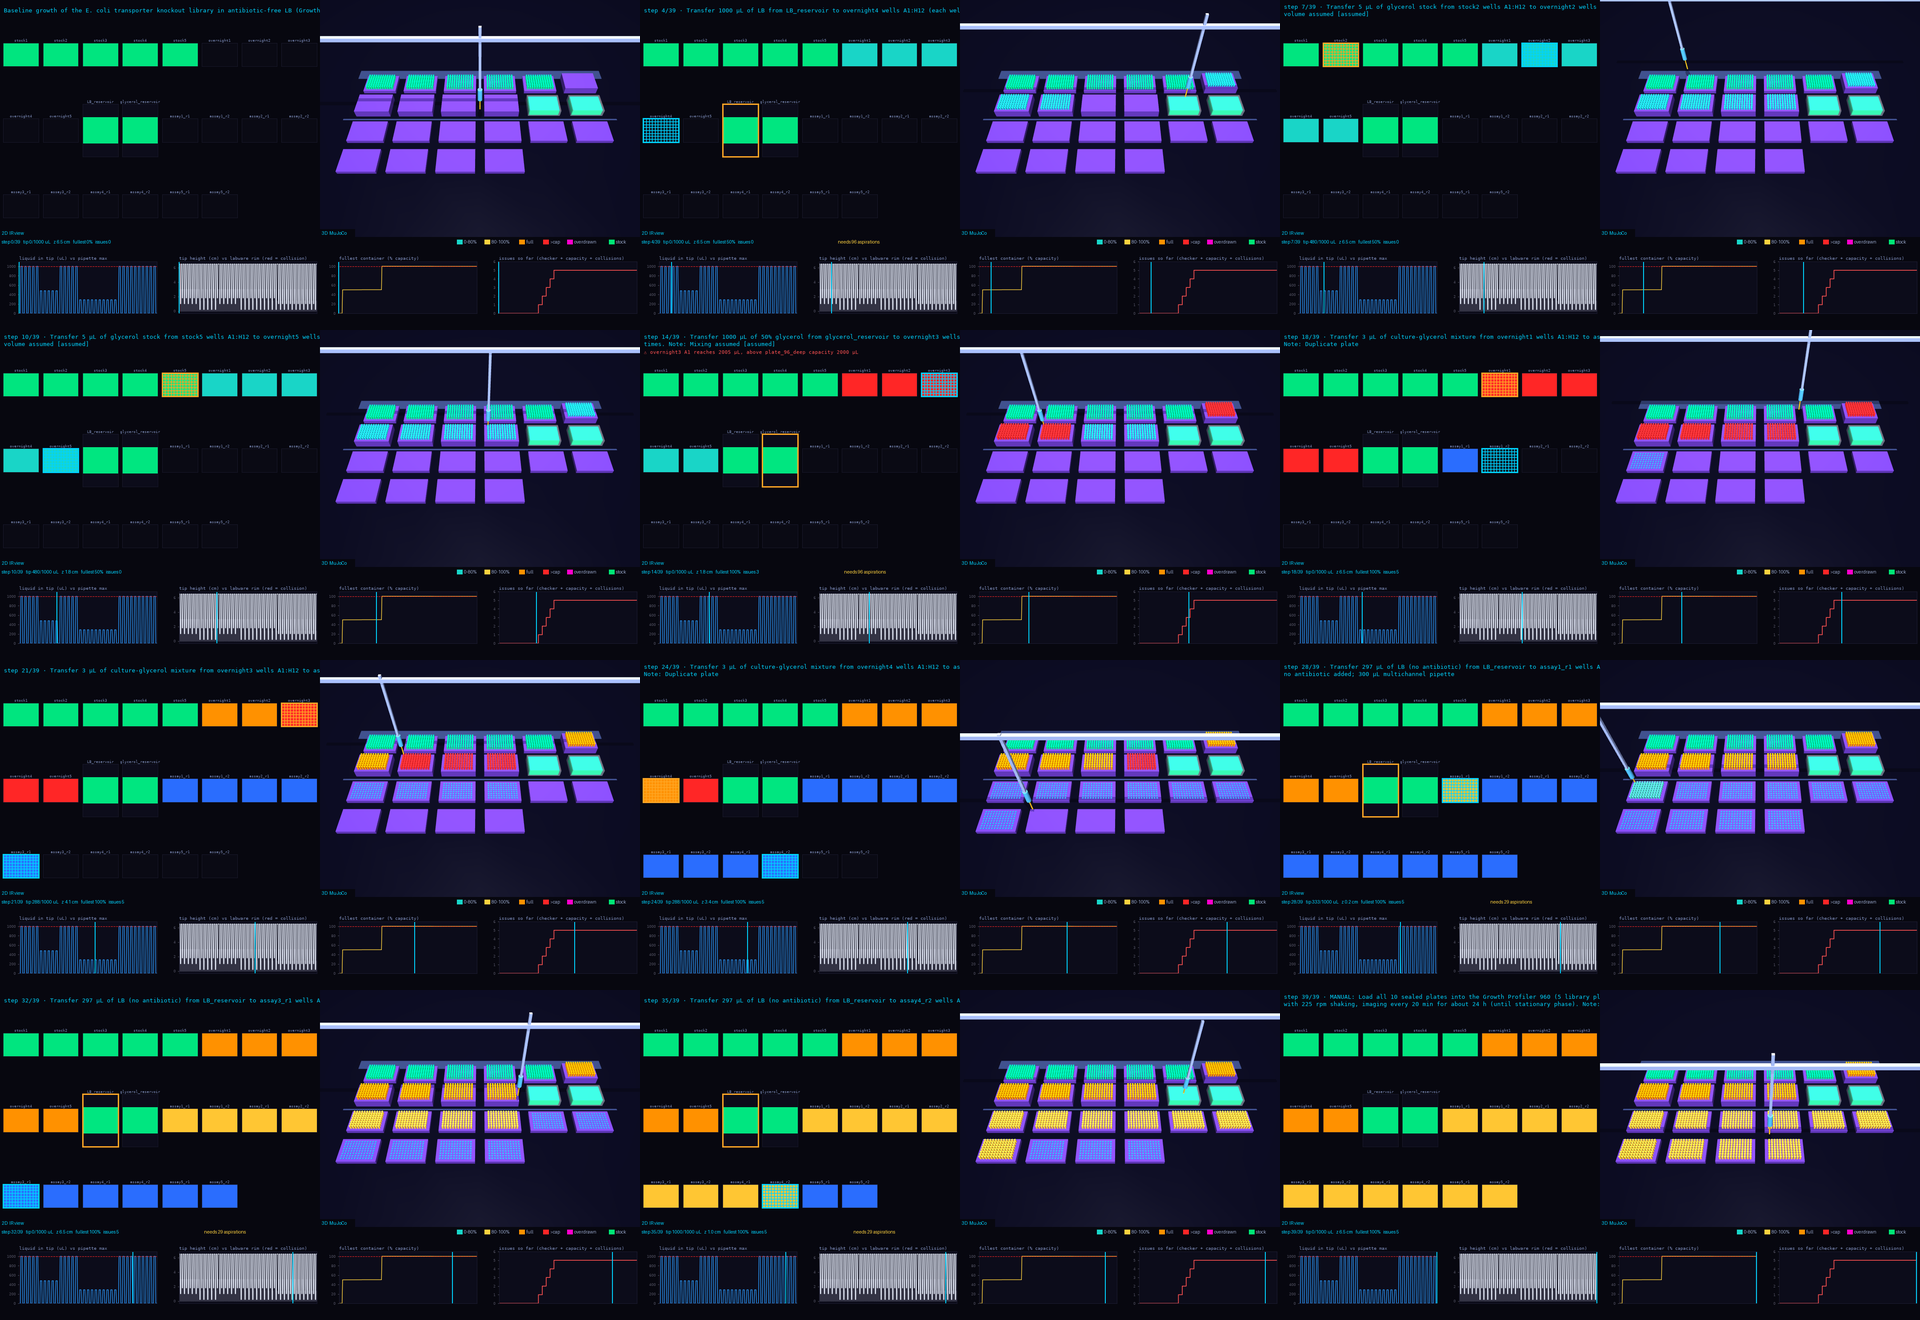
\includegraphics[width=0.92\textwidth]{../assets/examples3d/paper-10_3390_antibiotics11081129-exp1_frames.png}
\caption{MuJoCo 3D render strip: oracle trajectory (top) versus an agent
trajectory (bottom). Each column is a keyframe of the protocol execution.
Collision events and z-height violations are highlighted in red in the
collision-detection mode (not shown here).}
\label{fig:viz3d}
\end{figure}

% -----------------------------------------------------------------------
\section{Discussion}
\label{sec:discussion}
% -----------------------------------------------------------------------

\subsection{Interpretation}

The central finding is a \emph{capability split}: all evaluated models can
produce syntactically correct, simulator-passing OT-2 Python from a
plain-English task description, but none consistently encodes the tacit
wet-lab safety knowledge that a trained laboratory scientist would apply
automatically.
This split is consequential because the syntactic layer is what a naive
user would check---``did the code run?''---while the tacit layer contains
the errors that lead to failed experiments or, in clinical contexts,
diagnostic errors.

The phantom-mix finding is particularly noteworthy.
Standard microbiology training teaches that DNA should be gently mixed
into competent cells; but it also teaches that competent cells must not be
vortexed or mechanically stressed.
Two of three models applied the first heuristic without the second,
demonstrating over-application of a domain rule in a context where it is
contraindicated.

The universal elution-volume error in RNA extraction suggests that models
may default to the ``obvious'' value (the full elution volume) rather than
the conservative value specified in the source paper.
This is an instance of the general problem of specification fidelity under
distribution: the model knows the task, but its prior for the aspirate
volume (\textasciitilde100\,\textmu L for a 100\,\textmu L elution) is
stronger than the signal in the paper (\textasciitilde80\,\textmu L).

\subsection{Limitations}

\begin{enumerate}[leftmargin=*]
  \item \textbf{Small scale.} Seven tasks and one trial per model per task
    (pass@1) is too small for confident statistical conclusions.
    Variance estimates require pass@k with $k \geq 5$.

  \item \textbf{Single instrument class.} All tasks target the Opentrons
    OT-2.
    Generalisation to other liquid-handling platforms (Hamilton, Tecan,
    PyLabRobot-compatible instruments) is untested.

  \item \textbf{Simulator--reality gap.} The Opentrons simulator catches
    API-level errors but does not model true collisions, liquid physics
    (viscosity, surface tension), or labware geometry precisely.
    A protocol that passes simulation may still fail on a physical robot.

  \item \textbf{LLM-judge reproducibility.} The LLM judge introduces
    non-determinism.
    Rubric scores were collected from a single judge pass per trial;
    inter-judge agreement was not quantified.
    Future work should run multiple judge passes and report Krippendorff's
    $\alpha$.

  \item \textbf{No task-authoring bias control.} Several tasks were written
    by the same team that built the grader.
    An independent validation set authored by a separate team is needed.

  \item \textbf{End-state checks limited.} The deterministic end-state
    check applies to only two tasks where labware-to-instruction mapping is
    unambiguous.
    Extending it to multi-plate tasks requires publishing a full deck
    specification.
\end{enumerate}

\subsection{Future Work}

\begin{enumerate}[leftmargin=*]
  \item \textbf{Expand to 20+ tasks.} Priority targets include protein
    quantification (BCA/Bradford), cell-culture media preparation,
    nucleic-acid normalisation from Nanodrop readings, and ELISA plate
    washes.
  \item \textbf{Non-OT-2 instruments.} Extend the task suite to
    Hamilton STAR, Tecan Evo, and PyLabRobot-compatible devices.
  \item \textbf{Pass@k evaluation.} Run each task 10 times per model to
    report mean, variance, and pass@1, pass@3, pass@5.
  \item \textbf{Vagueness levels.} Introduce L0 (full specification),
    L1 (protocol omits one critical parameter), and L2 (protocol requires
    the model to resolve ambiguity via domain knowledge) versions of each
    task.
  \item \textbf{Multi-paper compound tasks.} Construct tasks that require
    synthesising information across two source papers, testing
    protocol-level reasoning rather than extraction.
  \item \textbf{End-to-end paper2protocol pipeline.} Evaluate the full
    pipeline (Figure~\ref{fig:pipeline}) starting from a DOI rather than
    a pre-written instruction, measuring the additional error introduced by
    the IR-extraction step.
\end{enumerate}

% -----------------------------------------------------------------------
\section{Conclusion}
\label{sec:conclusion}
% -----------------------------------------------------------------------

Text2WetLab establishes a reproducible evaluation framework for LLM agents
on the task of generating Opentrons OT-2 liquid-handling protocols from
plain-English instructions.
Across 21 trials spanning seven tasks and three frontier models, the key
finding is that syntactic correctness is no longer a differentiator at
current capability levels: all submissions passed the simulator.
Differentiation arises entirely from tacit wet-lab knowledge---tip
strategy, aspiration geometry, protocol fidelity, and the avoidance of
unrequested side-effects such as mixing competent cells.

Our dual-layer grading pipeline makes this distinction tractable.
The deterministic layer provides a reproducible, cost-free gate; the LLM
judge layer surfaces the domain-specific safety failures that would be
invisible without it.
We release all task definitions, grading code, and model trajectories under
open licenses to encourage community development of the benchmark.

From a practical standpoint, the results suggest that Sonnet~5.5 is the
most cost-effective choice for OT-2 protocol generation today, that no
single model dominates every task, and that human review of the tacit
safety dimensions remains essential before any model-generated protocol
is executed on a physical instrument.

% -----------------------------------------------------------------------
\section*{Acknowledgements}

The authors thank the developers of Harbor, Modal, Claude Code, and the
Opentrons open-source ecosystem.
The \texttt{opentrons-rna-extraction} oracle is the published script of
Steur et~al.\ (PLOS ONE, 2021)~\citep{steur2021hulp}.
The \texttt{golden-gate-assembly} task is derived from the AssemblyTron
experimental pipeline~\citep{assemblytron2023}.
The \texttt{colony-pcr-screening} task is inspired by the Slowpoke
workflow~\citep{slowpoke2025}.

% -----------------------------------------------------------------------
\section*{Data and Code Availability}

Task definitions, grading code, agent trajectories, and results are
available at \url{https://github.com/Tyronita/Text2WetLab} (private during
peer review; will be made public on acceptance).
The benchmark dataset is mirrored on the Hugging Face Hub.
All results reported in this paper are reproducible from the committed
\texttt{tasks/} directory using the commands in \texttt{README.md}.

% -----------------------------------------------------------------------
\section*{Author Contributions}

N.O'L.\ conceived the benchmark, designed the dual-layer grader,
and wrote the majority of the code and manuscript.
E.O'L.\ contributed to task design, grader validation, and manuscript review.
M.A.\ contributed to task sourcing and experimental validation.
L.S.\ contributed to system architecture and infrastructure.

% -----------------------------------------------------------------------
\section*{Competing Interests}

The authors declare no competing interests.

% -----------------------------------------------------------------------
\bibliographystyle{plainnat}
\bibliography{refs}

\end{document}
